\documentclass{standalone}
\usepackage{tikz}
\usetikzlibrary{patterns, positioning}
\usepackage[sfdefault]{ClearSans} %% option 'sfdefault' activates Clear Sans as the default text font
\usepackage[T1]{fontenc}

\begin{document}
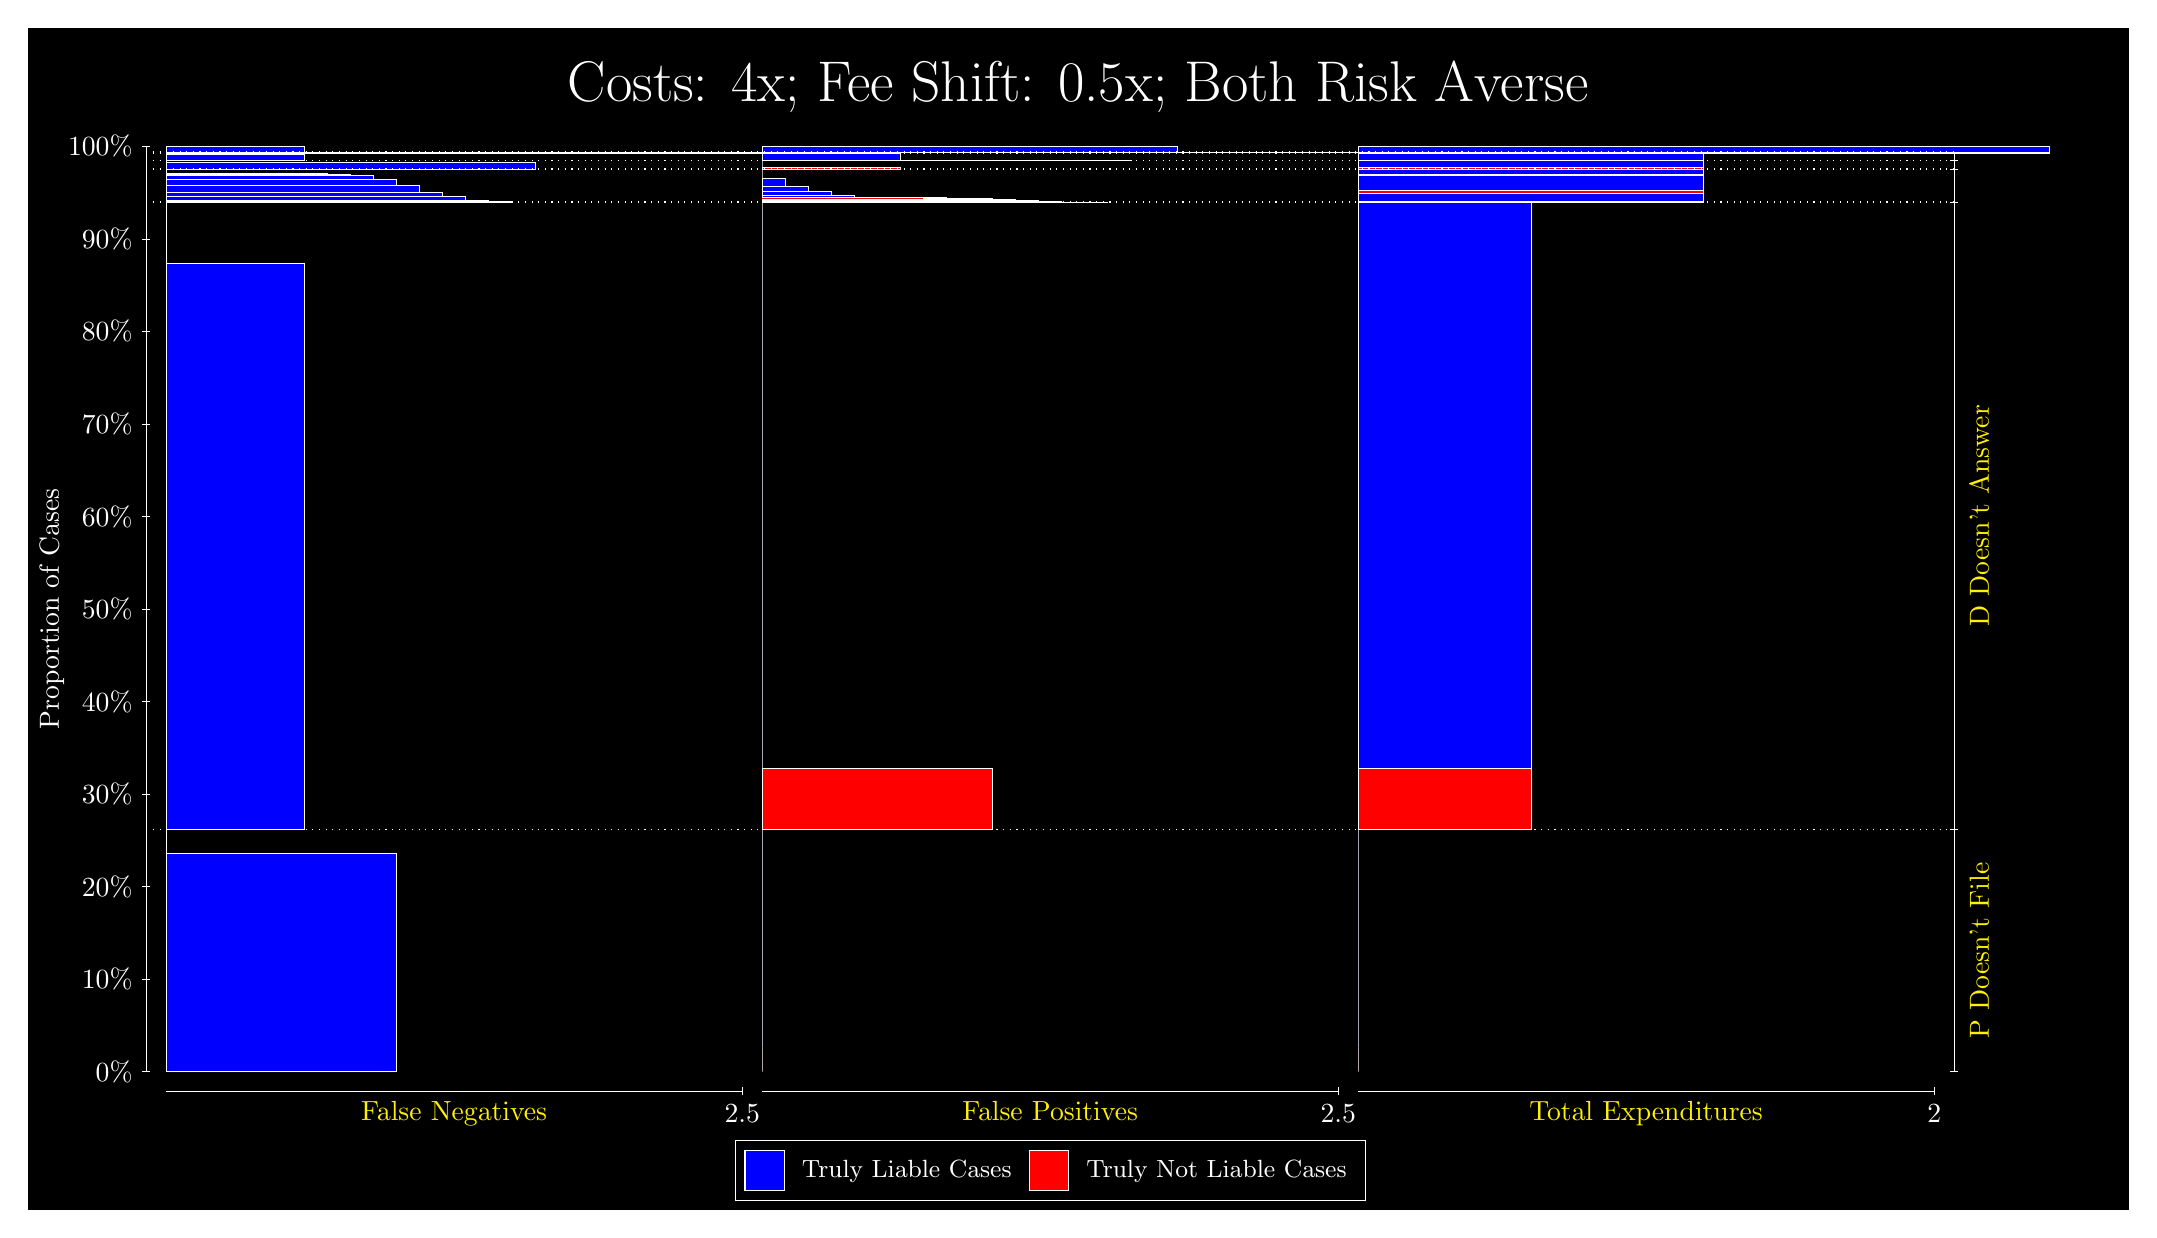
\begin{tikzpicture}
\draw[fill=black] (0,0) rectangle (26.667,15);
\draw[text=white] (0,13.5) rectangle (26.667,15) node[midway] {\huge Costs: 4x; Fee Shift: 0.5x; Both Risk Averse};
\draw[white, very thin] (1.5,1.75) -- (1.5,13.5);
\node[rotate=90, text=white, anchor=center] at (0.3, 7.625) {Proportion of Cases};
\draw[white, very thin] (1.45,1.75) -- (1.55,1.75);
\node[text=white, anchor=east] at (1.45, 1.75) {0\%};
\draw[white, very thin] (1.45,2.925) -- (1.55,2.925);
\node[text=white, anchor=east] at (1.45, 2.925) {10\%};
\draw[white, very thin] (1.45,4.1) -- (1.55,4.1);
\node[text=white, anchor=east] at (1.45, 4.1) {20\%};
\draw[white, very thin] (1.45,5.275) -- (1.55,5.275);
\node[text=white, anchor=east] at (1.45, 5.275) {30\%};
\draw[white, very thin] (1.45,6.45) -- (1.55,6.45);
\node[text=white, anchor=east] at (1.45, 6.45) {40\%};
\draw[white, very thin] (1.45,7.625) -- (1.55,7.625);
\node[text=white, anchor=east] at (1.45, 7.625) {50\%};
\draw[white, very thin] (1.45,8.8) -- (1.55,8.8);
\node[text=white, anchor=east] at (1.45, 8.8) {60\%};
\draw[white, very thin] (1.45,9.975) -- (1.55,9.975);
\node[text=white, anchor=east] at (1.45, 9.975) {70\%};
\draw[white, very thin] (1.45,11.15) -- (1.55,11.15);
\node[text=white, anchor=east] at (1.45, 11.15) {80\%};
\draw[white, very thin] (1.45,12.325) -- (1.55,12.325);
\node[text=white, anchor=east] at (1.45, 12.325) {90\%};
\draw[white, very thin] (1.45,13.5) -- (1.55,13.5);
\node[text=white, anchor=east] at (1.45, 13.5) {100\%};

\draw[white, very thin] (24.457,1.75) -- (24.457,13.5);
\draw[white, very thin] (24.407,1.75) -- (24.507,1.75);
\node[anchor=west] at (24.407, 1.75) {};
\draw[white, very thin] (24.407,4.8239) -- (24.507,4.8239);
\node[anchor=west] at (24.407, 4.8239) {};
\draw[white, very thin] (24.407,12.793) -- (24.507,12.793);
\node[anchor=west] at (24.407, 12.793) {};
\draw[white, very thin] (24.407,13.212) -- (24.507,13.212);
\node[anchor=west] at (24.407, 13.212) {};
\draw[white, very thin] (24.407,13.318) -- (24.507,13.318);
\node[anchor=west] at (24.407, 13.318) {};
\draw[white, very thin] (24.407,13.412) -- (24.507,13.412);
\node[anchor=west] at (24.407, 13.412) {};
\draw[white, very thin] (24.407,13.428) -- (24.507,13.428);
\node[anchor=west] at (24.407, 13.428) {};
\draw[white, very thin] (24.407,13.5) -- (24.507,13.5);
\node[anchor=west] at (24.407, 13.5) {};

\draw[white, very thin, fill=blue] (1.75,1.75) rectangle (4.6775,4.5165);
\draw[white, very thin, fill=red] (1.75,4.5165) rectangle (1.75,4.8239);
\draw[white, very thin, fill=blue] (1.75,4.8239) rectangle (3.5065,12.015);
\draw[white, very thin, fill=red] (1.75,12.015) rectangle (1.75,12.793);
\draw[white, very thin, fill=blue] (1.75,12.793) rectangle (6.1413,12.805);
\draw[white, very thin, fill=blue] (1.75,12.805) rectangle (5.8486,12.813);
\draw[white, very thin, fill=blue] (1.75,12.813) rectangle (5.5558,12.86);
\draw[white, very thin, fill=blue] (1.75,12.86) rectangle (5.2631,12.914);
\draw[white, very thin, fill=blue] (1.75,12.914) rectangle (4.9703,13.011);
\draw[white, very thin, fill=blue] (1.75,13.011) rectangle (4.6775,13.078);
\draw[white, very thin, fill=blue] (1.75,13.078) rectangle (4.3848,13.13);
\draw[white, very thin, fill=blue] (1.75,13.13) rectangle (4.092,13.147);
\draw[white, very thin, fill=blue] (1.75,13.147) rectangle (3.7993,13.156);
\draw[white, very thin, fill=red] (1.75,13.156) rectangle (1.75,13.212);
\draw[white, very thin, fill=blue] (1.75,13.212) rectangle (6.4341,13.296);
\draw[white, very thin, fill=red] (1.75,13.296) rectangle (1.75,13.318);
\draw[white, very thin, fill=blue] (1.75,13.318) rectangle (3.5065,13.405);
\draw[white, very thin, fill=red] (1.75,13.405) rectangle (1.75,13.412);
\draw[white, very thin, fill=blue] (1.75,13.412) rectangle (9.9471,13.424);
\draw[white, very thin, fill=red] (1.75,13.424) rectangle (1.75,13.428);
\draw[white, very thin, fill=blue] (1.75,13.428) rectangle (3.5065,13.499);
\draw[white, very thin, fill=red] (1.75,13.499) rectangle (1.75,13.5);
\draw[white, very thin, fill=red] (9.3189,1.75) rectangle (9.3189,2.0574);
\draw[white, very thin, fill=blue] (9.3189,2.0574) rectangle (9.3189,4.8239);
\draw[white, very thin, fill=red] (9.3189,4.8239) rectangle (12.246,5.6018);
\draw[white, very thin, fill=blue] (9.3189,5.6018) rectangle (9.3189,12.793);
\draw[white, very thin, fill=red] (9.3189,12.793) rectangle (13.71,12.794);
\draw[white, very thin, fill=red] (9.3189,12.794) rectangle (13.417,12.795);
\draw[white, very thin, fill=red] (9.3189,12.795) rectangle (13.125,12.8);
\draw[white, very thin, fill=red] (9.3189,12.8) rectangle (12.832,12.812);
\draw[white, very thin, fill=red] (9.3189,12.812) rectangle (12.539,12.825);
\draw[white, very thin, fill=red] (9.3189,12.825) rectangle (12.246,12.834);
\draw[white, very thin, fill=red] (9.3189,12.834) rectangle (11.954,12.846);
\draw[white, very thin, fill=red] (9.3189,12.846) rectangle (11.661,12.847);
\draw[white, very thin, fill=red] (9.3189,12.847) rectangle (11.368,12.849);
\draw[white, very thin, fill=blue] (9.3189,12.849) rectangle (10.783,12.858);
\draw[white, very thin, fill=blue] (9.3189,12.858) rectangle (10.49,12.874);
\draw[white, very thin, fill=blue] (9.3189,12.874) rectangle (10.197,12.927);
\draw[white, very thin, fill=blue] (9.3189,12.927) rectangle (9.9044,12.994);
\draw[white, very thin, fill=blue] (9.3189,12.994) rectangle (9.6116,13.091);
\draw[white, very thin, fill=blue] (9.3189,13.091) rectangle (9.3189,13.212);
\draw[white, very thin, fill=red] (9.3189,13.212) rectangle (11.075,13.233);
\draw[white, very thin, fill=blue] (9.3189,13.233) rectangle (9.3189,13.318);
\draw[white, very thin, fill=red] (9.3189,13.318) rectangle (14.003,13.324);
\draw[white, very thin, fill=blue] (9.3189,13.324) rectangle (11.075,13.412);
\draw[white, very thin, fill=red] (9.3189,13.412) rectangle (11.075,13.416);
\draw[white, very thin, fill=blue] (9.3189,13.416) rectangle (9.3189,13.428);
\draw[white, very thin, fill=red] (9.3189,13.428) rectangle (17.516,13.429);
\draw[white, very thin, fill=blue] (9.3189,13.429) rectangle (14.588,13.5);
\draw[white, very thin, fill=red] (16.888,1.75) rectangle (16.888,2.0574);
\draw[white, very thin, fill=blue] (16.888,2.0574) rectangle (16.888,4.8239);
\draw[white, very thin, fill=red] (16.888,4.8239) rectangle (19.083,5.6018);
\draw[white, very thin, fill=blue] (16.888,5.6018) rectangle (19.083,12.793);
\draw[white, very thin, fill=red] (16.888,12.793) rectangle (21.279,12.806);
\draw[white, very thin, fill=blue] (16.888,12.806) rectangle (21.279,12.903);
\draw[white, very thin, fill=red] (16.888,12.903) rectangle (21.279,12.94);
\draw[white, very thin, fill=blue] (16.888,12.94) rectangle (21.279,13.137);
\draw[white, very thin, fill=red] (16.888,13.137) rectangle (21.279,13.143);
\draw[white, very thin, fill=blue] (16.888,13.143) rectangle (21.279,13.212);
\draw[white, very thin, fill=red] (16.888,13.212) rectangle (21.279,13.233);
\draw[white, very thin, fill=blue] (16.888,13.233) rectangle (21.279,13.318);
\draw[white, very thin, fill=red] (16.888,13.318) rectangle (21.279,13.324);
\draw[white, very thin, fill=blue] (16.888,13.324) rectangle (21.279,13.412);
\draw[white, very thin, fill=red] (16.888,13.412) rectangle (25.67,13.416);
\draw[white, very thin, fill=blue] (16.888,13.416) rectangle (25.67,13.428);
\draw[white, very thin, fill=red] (16.888,13.428) rectangle (25.67,13.429);
\draw[white, very thin, fill=blue] (16.888,13.429) rectangle (25.67,13.5);
\draw[white, dotted] (1.5,4.8239) -- (24.457,4.8239);
\draw[white, dotted] (1.5,12.793) -- (24.457,12.793);
\draw[white, dotted] (1.5,13.212) -- (24.457,13.212);
\draw[white, dotted] (1.5,13.318) -- (24.457,13.318);
\draw[white, dotted] (1.5,13.412) -- (24.457,13.412);
\draw[white, dotted] (1.5,13.428) -- (24.457,13.428);
\draw[white, very thin] (1.75,1.5) -- (9.0689,1.5);
\node[text=yellow, anchor=north] at (5.4094, 1.5) {False Negatives};
\draw[white, very thin] (9.0689,1.45) -- (9.0689,1.55);
\node[text=white, anchor=north] at (9.0689, 1.45) {2.5};

\draw[white, very thin] (9.3189,1.5) -- (16.638,1.5);
\node[text=yellow, anchor=north] at (12.978, 1.5) {False Positives};
\draw[white, very thin] (16.638,1.45) -- (16.638,1.55);
\node[text=white, anchor=north] at (16.638, 1.45) {2.5};

\draw[white, very thin] (16.888,1.5) -- (24.207,1.5);
\node[text=yellow, anchor=north] at (20.547, 1.5) {Total Expenditures};
\draw[white, very thin] (24.207,1.45) -- (24.207,1.55);
\node[text=white, anchor=north] at (24.207, 1.45) {2};

\node[text=yellow, centered, rotate=90] at (24.777, 3.2869) {P Doesn't File};
\node[text=yellow, centered, rotate=90] at (24.777, 8.8083) {D Doesn't Answer};






\draw (12.978300999999998,1.5) node[draw=none] (baseCoordinate) {};
\begin{scope}[align=center]
        \matrix[scale=0.5, draw=white, below=0.5cm of baseCoordinate, nodes={draw}, column sep=0.1cm]{
            \node[rectangle, draw, minimum width=0.5cm, minimum height=0.5cm, fill=blue] {}; &
            \node[draw=none, font=\small, text=white] (B) {Truly Liable Cases}; &
            \node[rectangle, draw, minimum width=0.5cm, minimum height=0.5cm, fill=red] {}; &
            \node[draw=none, font=\small, text=white] (B) {Truly Not Liable Cases}; \\
            };
\end{scope}

\end{tikzpicture}
\end{document}